\chapter{Content-based image retrieval}

Image retrieval has been an active research field since the 1970s. The traditional approaches included manual annotation of the images by textual or numerical metadata. The user could then formulate a query against these annotations to retrieve relevant images. This approach is often referred to as Concept-based image retrieval.

There are several drawbacks to the textual or numerical annotations. First of all, extensive human annotations are often needed to provide rich data for filtering. Including also spatial information of the objects takes more resources than only writing down present objects in the image. Furthermore, the images often include too many details (i.e. type, color, or shape of the objects), which may be impossible to comprehend by manual annotations.  The annotations may not even represent a stable truth. With a different annotator, the annotations may include different details/objects, which were perceived differently. When user searches for an image, she has to know the exact terms the annotators used in order to be able to retrieve the images they want. As the last problem, we pose with human annotations is the scalability. As the amount of information increases every second, there is no human capability to hand process all the examples.

During the 1990s, content-based image retrieval (CBIR) emerged. In the CBIR approach, the images are indexed by features directly derived from their visual content using automatic or semi-automatic image processing techniques. Such indexing lacks building blocks (for example verbal description), on the other hand, provides semantic information about the whole images or its regions. The attributes of images are complex functions of regions of the image or the whole image.

CBIR has received considerable research interest in the last decades. With the advancement in Deep Learning, a new pool of possible complex functions to describe the images emerged. In our solutions, we use pre-trained neural networks to extract features. Based on these features, we implemented and evaluated several approaches to the CBIR task.

Our solutions are focused on the known-item search task. An alternative could be an Ad Hoc search, which goal is to retrieve all relevant items to the query. Known-item search task rather works with retrieving a specific item from the dataset, which is known.

Following this chapter, we continue with specific solutions implemented in this thesis. Here we formulate the task and the goal.

\section*{Task formulation and evaluation}

As our inputs we have a database of items and the query. Since we work with known-item search task, the query is also present in the database. Our goal is to order the items in the database in such way, that the query has the lowest rank. Alternatively said, if we order based on the similarity, we aim for the request and query image to have the highest similarity. We refer to the position of our query in ranked results as \emph{rank}.

Our goal is to developed a solution, which minimises the rank of the query. In the following chapters we aim to test two different possibilities how to describe a query to the system.

We also provide a numerical comparison of the performance of different setups. To provide a comparison we a \emph{Rank of searched item}. The graphs contain the amount of requests solved in a given rank. In all graphs we refer to a rank as a percentage of the dataset. The amount of requests solved is also expressed as the percentage.

We use a figure \ref{fig:mobilenet_whole_image_example} as an example to explain the graphs we will use for evaluation of the performance of the system. In this specific case 90\% of annotated collages are ranked below 50\% of the database. This can be also said in other words, that in 90\% of cases by stating a query we were able to eliminate half of the dataset as unrelated. We can also notice a steep curve in the beginning. It shows 70\% of the collages were ranked in the first 10\% of the database. We can see that this particular system worked well for 70\% of the collages well, but struggled with the rest of the dataset.

\begin{figure}
    \centering
    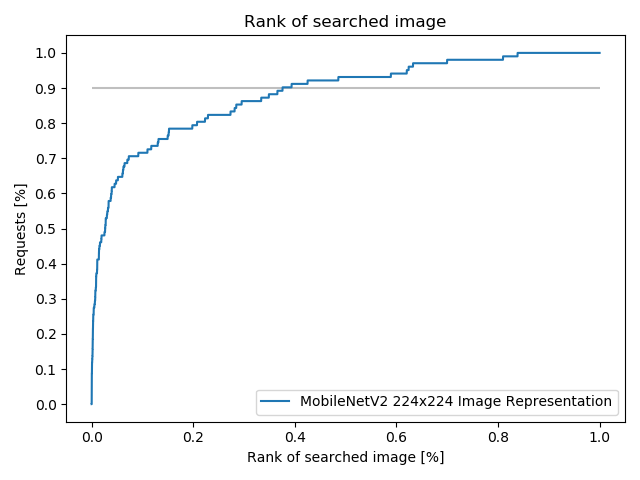
\includegraphics[width=0.8\linewidth]{img/mobilenet_whole_image.png}
    \caption{Performance of MobileNetV2 on annotated collages}
    \label{fig:mobilenet_whole_image_example}
\end{figure}

For these evaluations we use annotated queries. We described them in the section \ref{s:dataset}.